\message{ !name(paper.tex)}%  article.tex (Version 3.3, released 19 January 2008)
%  Article to demonstrate format for SPIE Proceedings
%  Special instructions are included in this file after the
%  symbol %>>>>
%  Numerous commands are commented out, but included to show how
%  to effect various options, e.g., to print page numbers, etc.
%  This LaTeX source file is composed for LaTeX2e.

%  The following commands have been added in the SPIE class 
%  file (spie.cls) and will not be understood in other classes:
%  \supit{}, \authorinfo{}, \skiplinehalf, \keywords{}
%  The bibliography style file is called spiebib.bst, 
%  which replaces the standard style unstr.bst.  

\documentclass[]{spie}  %>>> use for US letter paper
%%\documentclass[a4paper]{spie}  %>>> use this instead for A4 paper
%%\documentclass[nocompress]{spie}  %>>> to avoid compression of citations
%% \addtolength{\voffset}{9mm}   %>>> moves text field down
%% \renewcommand{\baselinestretch}{1.65}   %>>> 1.65 for double spacing, 1.25 for 1.5 spacing 
%  The following command loads a graphics package to include images 
%  in the document. It may be necessary to specify a DVI driver option,
%  e.g., [dvips], but that may be inappropriate for some LaTeX 
%  installations. 
\usepackage{graphicx}
\usepackage{subfig}
\usepackage{caption}
\usepackage{subcaption}

\title{Texture mapping 3D planar models of indoor environments with noisy camera poses} 

%>>>> The author is responsible for formatting the 
%  author list and their institutions.  Use  \skiplinehalf 
%  to separate author list from addresses and between each address.
%  The correspondence between each author and his/her address
%  can be indicated with a superscript in italics, 
%  which is easily obtained with \supit{}.

\author{Peter Cheng, Michael Anderson, Stewart He, Avideh Zakhor
\skiplinehalf
University of California, Berkeley\\
}

 

%%%%%%%%%%%%%%%%%%%%%%%%%%%%%%%%%%%%%%%%%%%%%%%%%%%%%%%%%%%%% 
%>>>> uncomment following for page numbers
% \pagestyle{plain}    
%>>>> uncomment following to start page numbering at 301 
%\setcounter{page}{301} 
 
\begin{document}

\message{ !name(paper.tex) !offset(674) }
\subsection{Future stuff}
For the sake of simplicity, - cases where multiple whatever are few,
but for true generality, should go to 3d adjustments


\begin{figure*}
  \centering
  \subfloat[][]{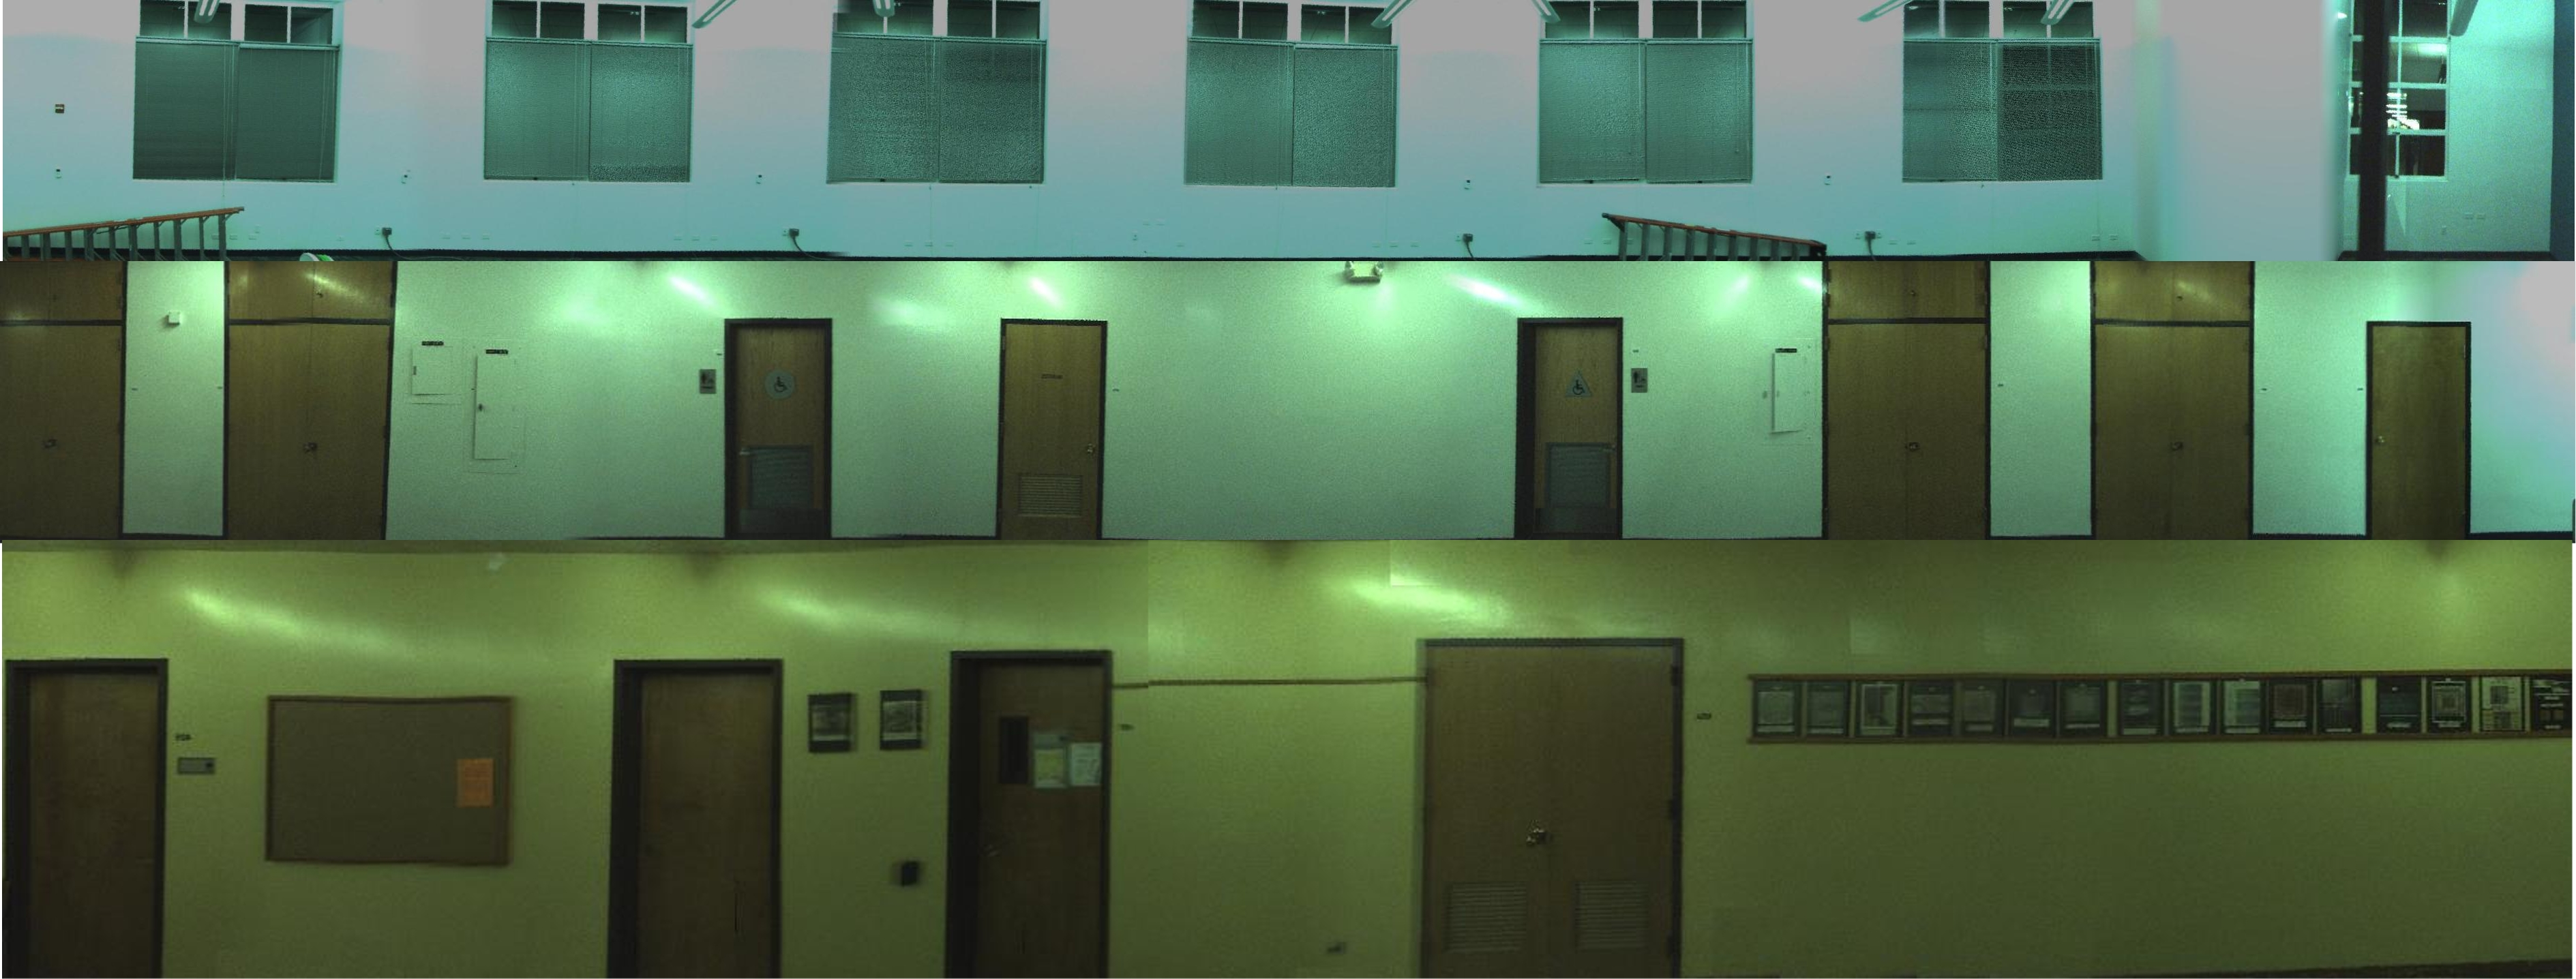
\includegraphics[width=3in]{finalfloors.jpg}}
  ~~~~~~~~
  \centering
  \subfloat[][]{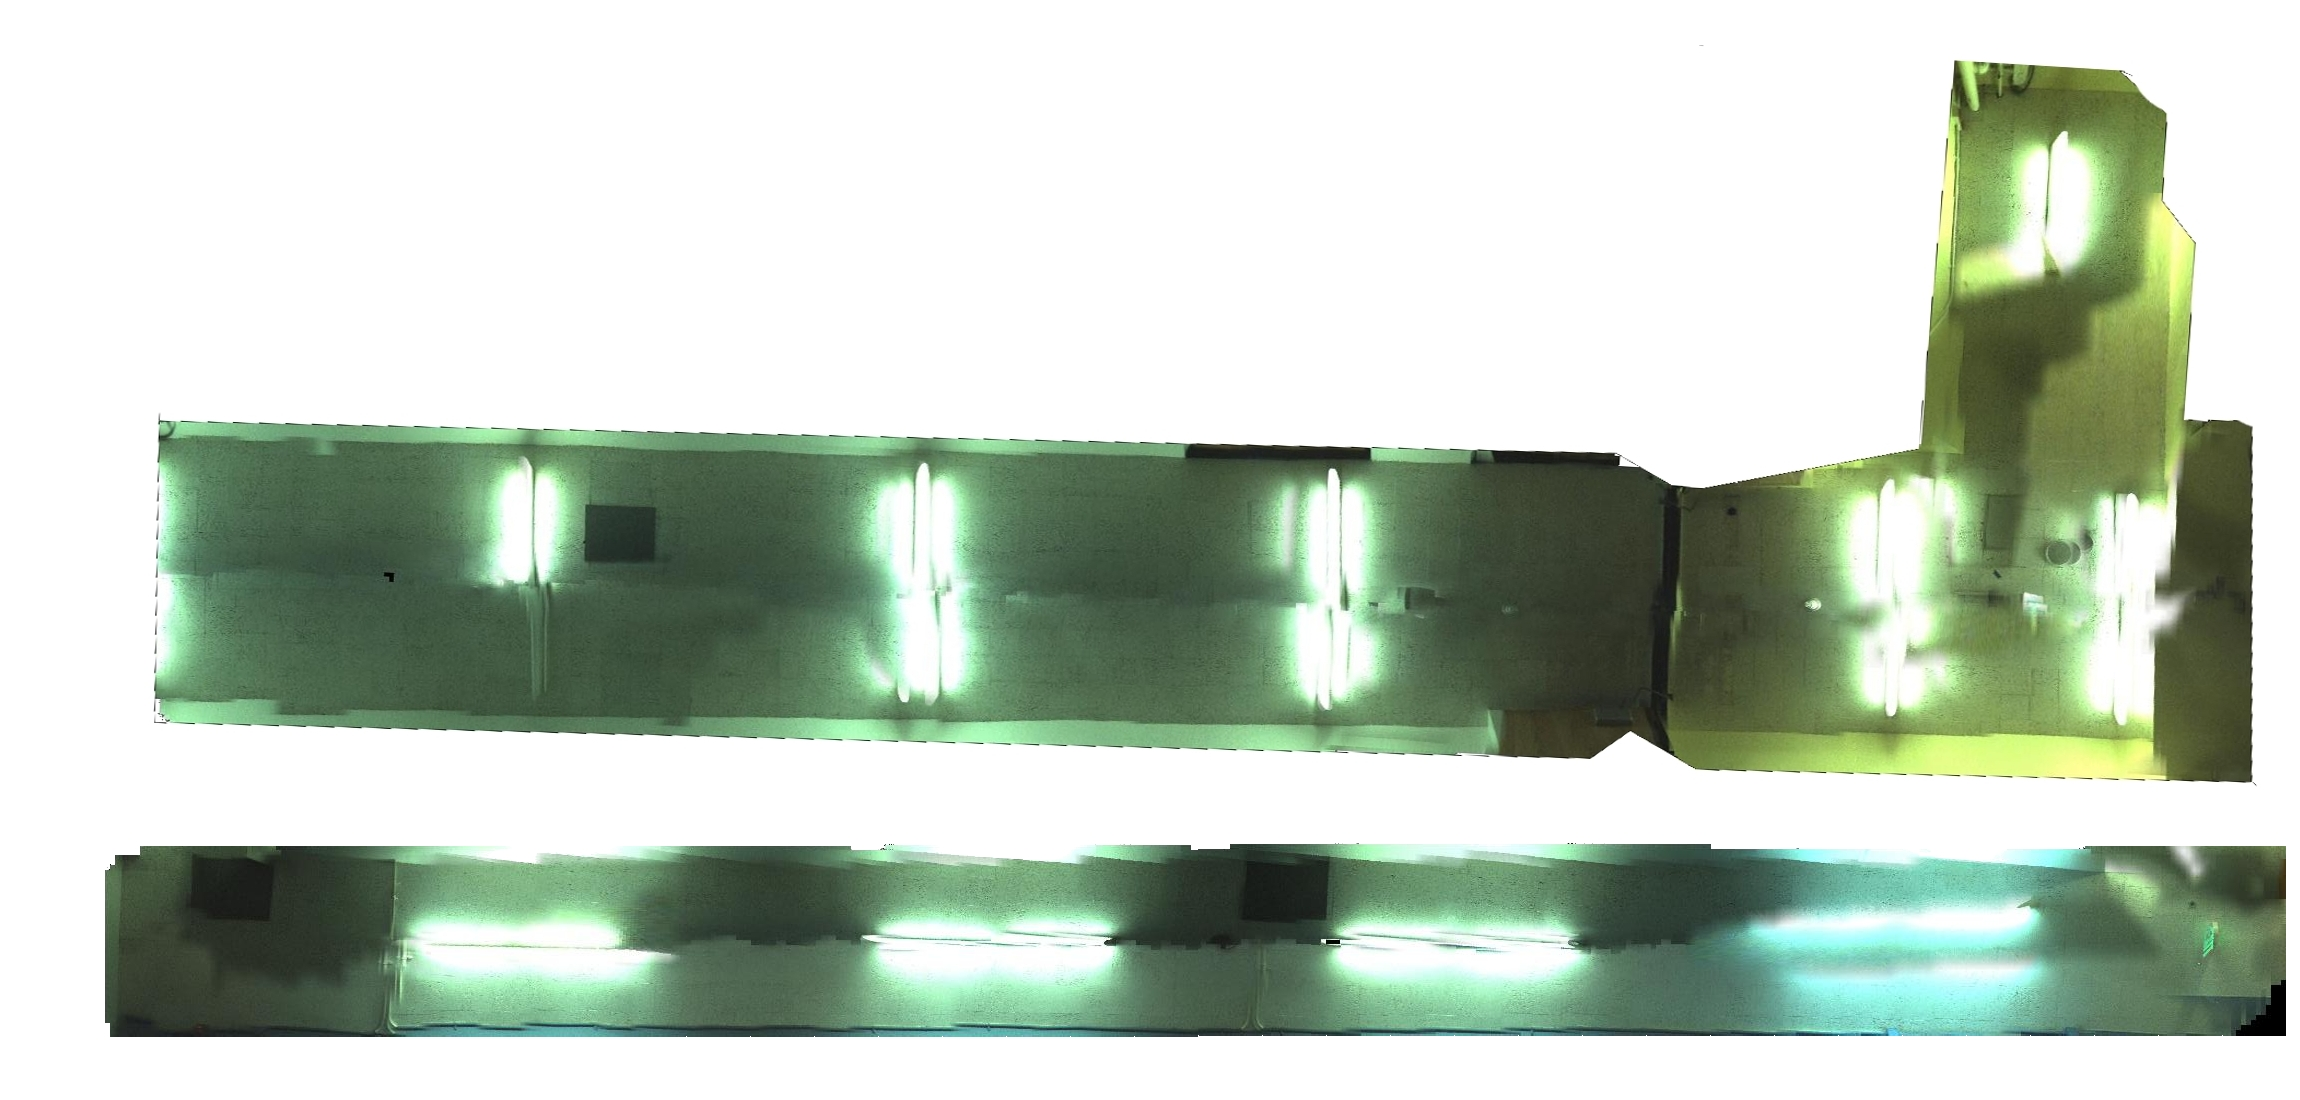
\includegraphics[width=3in]{finalceilings.jpg}}

  \centering 
  \subfloat[][]{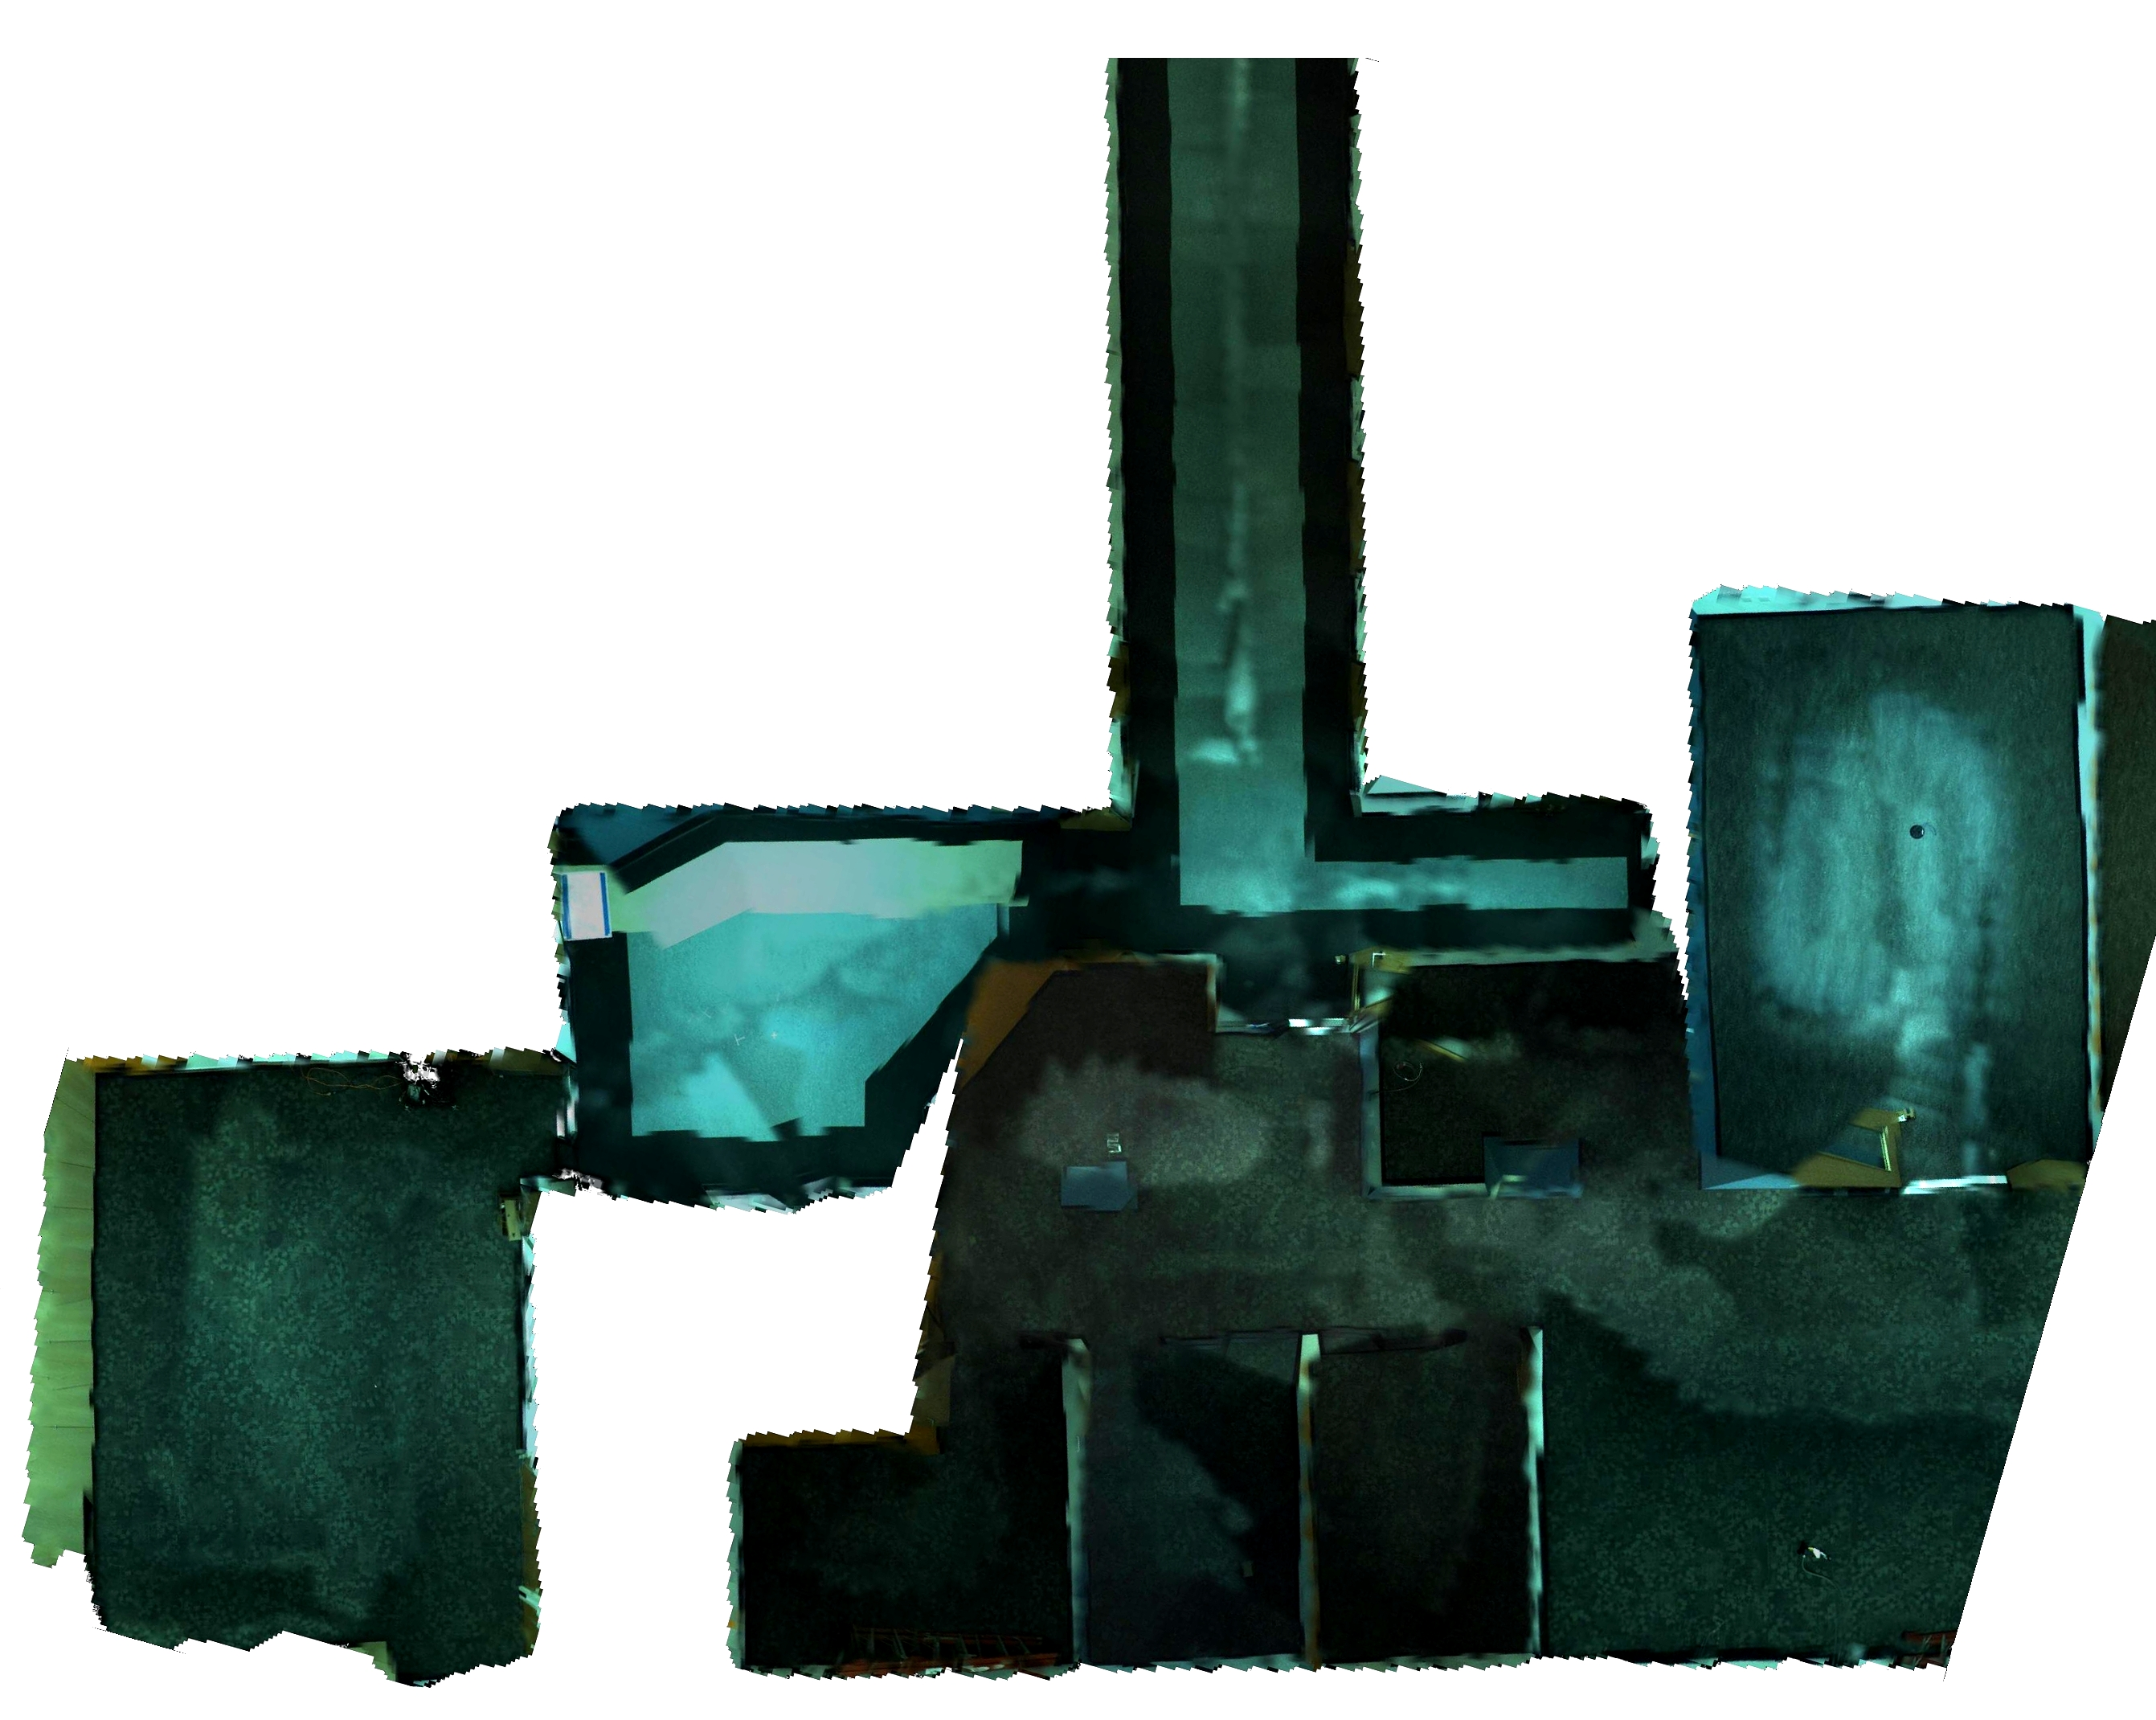
\includegraphics[height=2in, width=3in]{floorcropped.jpg}}
  ~~~~~~~~
  \centering
  \subfloat[][]{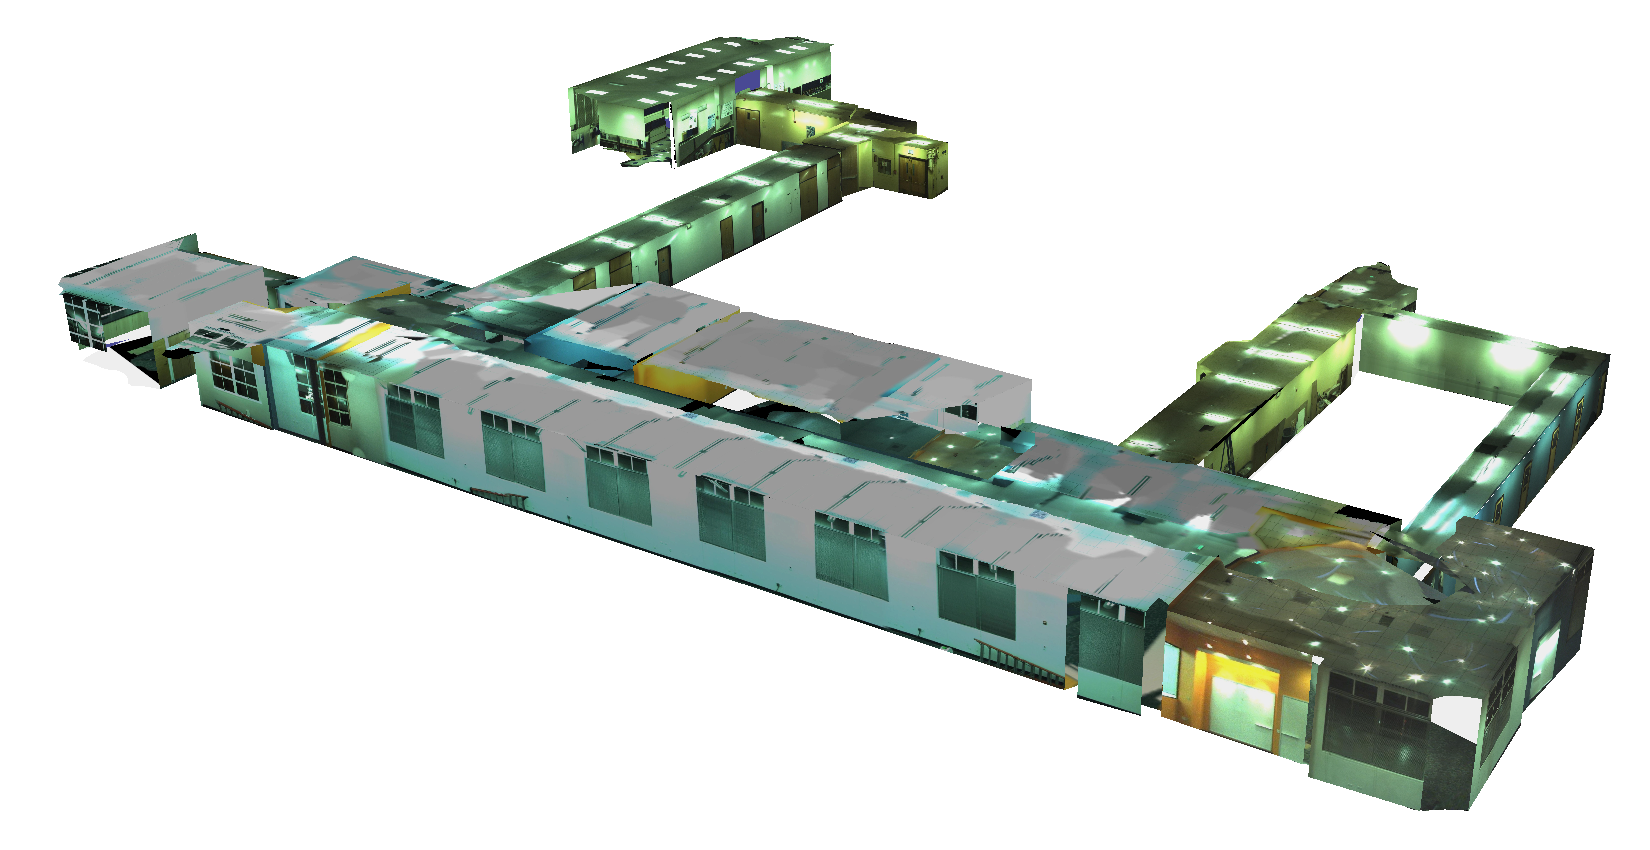
\includegraphics[width=3in]{fullmodel.png}}
  \caption{Examples of our final texture mapping output for (a) walls,
    (b) ceilings, (c) an entire floor, (d) a full model.}
  \label{fig:results}
\end{figure*}


%%%%%%%%%%%%%%%%%%%%%%%%%%%%%%%%%%%%%%%%%%%%%%%%%%%%%%%%%%%%%
%%%%% References %%%%%

\bibliography{report} %>>>> bibliography data in report.bib
\bibliographystyle{spiebib} %>>>> makes bibtex use spiebib.bst

\message{ !name(paper.tex) !offset(672) }

\end{document} 
